\chapter{固有距離、クルスカル幾何、そして事象の地平面の観測者}

シュヴァルツシルト計量は地平面で特異になるように見える。曲率はそうではない。この二つの主張を区別するために、まずブラックホールの全体の大きさを取り除き、次に動径座標を地平面からの固有距離で置き換える。地平面の近くでは、得られる幾何は加速座標で書かれた通常の平坦な時空である。その幾何が描かれてしまえば、アリス、ボブ、チャーリーに関する問いは、言葉のパラドックスではなく世界線と光線に関する問いになる。

\section{シュヴァルツシルト半径をスケールアウトする}

まずプライム付き座標から始める。そうすれば、再スケールされた変数が後に馴染みのある名前を持てる：
\begin{equation}
d\tau^2
=
\left(1-\frac{2MG}{r'}\right)dt'^2
-
\frac{dr'^2}{1-\frac{2MG}{r'}}
-
r'^2d\Omega_2^2.
\label{eq:l7-schwarzschild-dimensional}
\end{equation}
シュヴァルツシルト半径と無次元座標を導入する：
\begin{equation}
r_{\mathrm S}=2MG,
\qquad
r=\frac{r'}{r_{\mathrm S}},
\qquad
t=\frac{t'}{r_{\mathrm S}}.
\label{eq:l7-rescaling}
\end{equation}
ここでは\(c=1\)を用いるので、時間と長さは同じ単位を持つ。したがって半径\(r_{\mathrm S}\)は長さであり、かつその長さに付随する光の横断時間でもある。代入すると
\begin{equation}
d\tau^2
=r_{\mathrm S}^2
\left[
\left(1-\frac1r\right)dt^2
-
\frac{dr^2}{1-\frac1r}
-
r^2d\Omega_2^2
\right].
\label{eq:l7-schwarzschild-rescaled}
\end{equation}
となる。したがって、すべての非回転・非帯電のシュヴァルツシルトブラックホールは同じ無次元幾何を持つ。質量を変えると、計量に掛かる物差しが変わるのであり、括弧内の式の形は変わらない。状況は、すべての距離を球の半径で割った後に球を描くことに似ている。同じ図が月と地球を記述するが、一方の図の1センチメートルは異なる物理的距離を表す。

\begin{classroomqa}
\audiencequestion{計量の動径部分と角度部分にはどちらの符号が属するのか。}
\lecturerresponse{ここで用いている\(+---\)の符号規則では、空間部分の両方が負号を持つ。式を書いている間に、その符号が教室で話題になった。角度因子は、極座標が軸から測られるか赤道から測られるかに応じてサインまたはコサインを用いることができる。コンパクトな表記\(d\Omega_2^2\)はその規約の問題を避ける。
\lecturetimestamp{00:07:48--00:08:12}}
\end{classroomqa}

\section{地平面における曲率スケール}

この再スケーリングは、長いテンソル計算なしに重要な物理的問いに答える。計量の成分は無次元である。クリストッフェル記号は座標微分を一つ含むため、逆長さの次元を持ち、物理的な正規直交枠におけるリーマンテンソルの成分は次元
\begin{equation}
[g_{\mu\nu}]=1,
\qquad
[\Gamma^\mu{}_{\nu\rho}]=L^{-1},
\qquad
[R_{\hat\alpha\hat\beta\hat\gamma\hat\delta}]
=L^{-2}.
\label{eq:l7-curvature-dimensions}
\end{equation}
を持つ。地平面\(r=1\)では、利用可能な唯一の物理的長さは\(r_{\mathrm S}\)である。したがって潮汐曲率スケールは
\begin{equation}
\left|R_{\hat\alpha\hat\beta\hat\gamma\hat\delta}\right|_{\mathrm{hor}}
\sim \frac{1}{r_{\mathrm S}^2}.
\label{eq:l7-horizon-curvature}
\end{equation}
でなければならない。より一般には、それは\(r_{\mathrm S}^{-2}\)に\(r\)の無次元関数を掛けたものである。この主張はリーマン潮汐場に関するものであり、シュヴァルツシルト真空で消えるリッチスカラーに関するものではない。

物理的結論は直ちに得られる。質量を増やすと\(r_{\mathrm S}\)が増大し、地平面における潮汐場は弱まる。小さなブラックホールは、物体が横切る間に広がった物体を引き裂くことができる。超大質量ブラックホールの地平面近くでは、潮汐力は穏やかであり得る。それにもかかわらず曲率は内側へ向かって増大し、\(r=0\)で発散する。したがって地平面と特異点は根本的に異なる対象である。

\section{地平面からの固有距離}

残りの局所計算では、\(r_{\mathrm S}=1\)と置く。相対性理論において座標変換は見かけの問題ではない。不適切な座標は、正則な幾何を特異な係数の背後に隠し得る。シュヴァルツシルト座標差\(r-1\)は、地平面からの測定された動径距離ではない。

\begin{figure}[htbp]
\centering
\includegraphics[width=0.78\textwidth]{lecture_07_figure_02.png}
\caption{黒板で用いられた動径座標線。地平面は\(r=1\)にあり、一方\(r=0\)は曲率特異点である。}
\lectureframe{00:16:11}
\end{figure}

\(t\)と角度を固定する。そのとき正の空間線素は
\begin{equation}
ds^2=\frac{dr^2}{1-\frac1r},
\qquad
ds=\sqrt{\frac{r}{r-1}}\,dr.
\label{eq:l7-radial-proper-line}
\end{equation}
である。地平面からの無次元固有距離を
\begin{equation}
\rho(r)
=
\int_1^r\sqrt{\frac{r'}{r'-1}}\,dr'.
\label{eq:l7-rho-definition}
\end{equation}
で定義する。全体のスケールを戻すと、物理的距離は\(r_{\mathrm S}\rho\)である。積分の閉じた形は必要ない。必要なのはその導関数だけである：
\begin{equation}
\frac{d\rho}{dr}
=\sqrt{\frac{r}{r-1}},
\qquad
d\rho^2
=\frac{dr^2}{1-\frac1r}.
\label{eq:l7-rho-derivative}
\end{equation}
したがって複雑な動径項はちょうど\(-d\rho^2\)になる。この単純化が\(\rho\)を導入する理由である。

ここで時間座標をもう一度再スケールする：
\begin{equation}
\omega=\frac{t}{2}.
\label{eq:l7-omega}
\end{equation}
\(r\)は\(\rho\)の関数であるから、計量は
\begin{equation}
d\tau^2
=
F(\rho)\rho^2d\omega^2
-
d\rho^2
-
r(\rho)^2d\Omega_2^2.
\label{eq:l7-rho-metric}
\end{equation}
と書ける。

\begin{classroomqa}
\audiencequestion{時間の係数が\(F(\rho)\rho^2\)の形を持つように、単に\(F(\rho)\)を定義しているのか。}
\lecturerresponse{はい。この時点では、この因子分解には独立した物理的内容はない。それは便利な定義である。その有用性は、\(F\)の極限を地平面の近くと遠方で取るときに現れる。
\lecturetimestamp{00:26:39--00:26:59}}
\end{classroomqa}

遠方では、シュヴァルツシルト時間の係数は1に近づく。\(dt=2d\omega\)であるから、これは
\begin{equation}
\lim_{\rho\to\infty}F(\rho)\rho^2=4.
\label{eq:l7-far-limit}
\end{equation}
となる。地平面の近くでは、式~\eqref{eq:l7-rho-definition}より
\begin{equation}
\begin{aligned}
\rho&\simeq 2\sqrt{r-1},\\
r(\rho)&=1+\frac{\rho^2}{4}+O(\rho^4),\\
\lim_{\rho\to0}F(\rho)&=1.
\end{aligned}
\label{eq:l7-near-expansion}
\end{equation}

\begin{figure}[htbp]
\centering
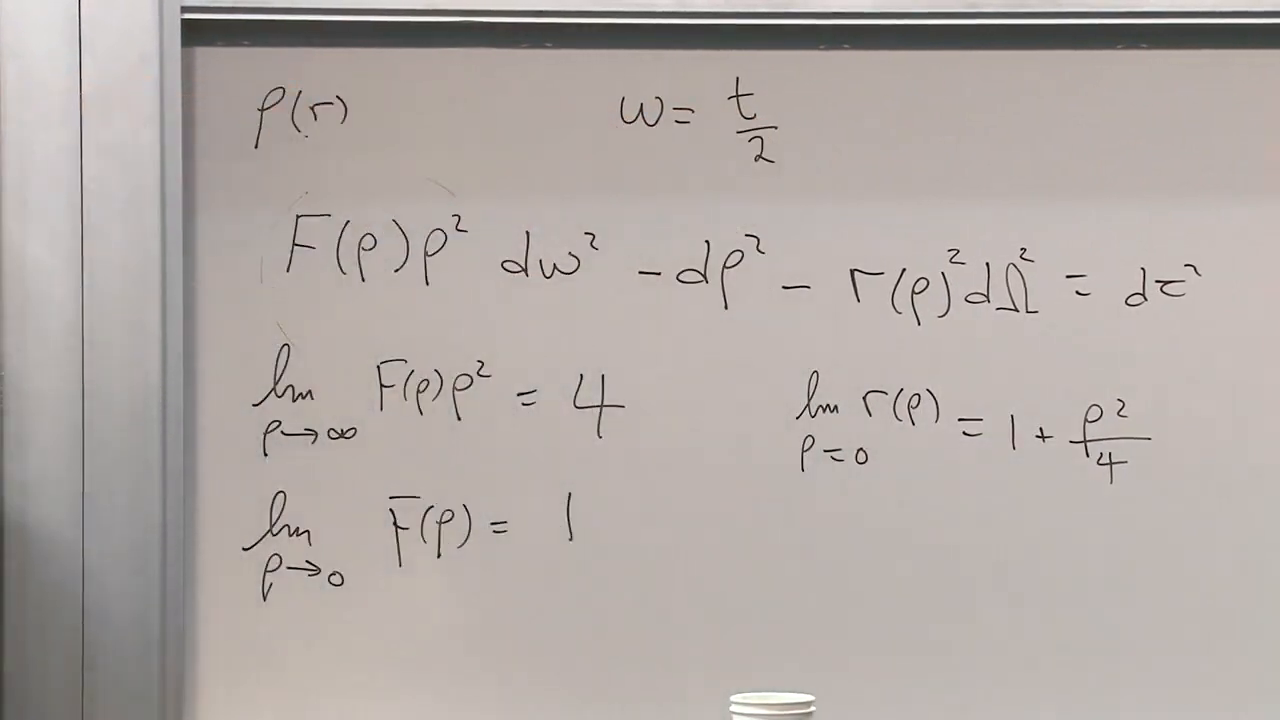
\includegraphics[width=0.90\textwidth]{lecture_07_figure_03.png}
\caption{\((\rho,\omega)\) における計量、その漸近的時間係数、および近地平極限 \(F\to1\) と \(r=1+\rho^2/4+\cdots\)。}
\lectureframe{00:37:30}
\end{figure}

\section{地平線に隠された平坦時空}

\(\rho=0\) の近くで、式~\eqref{eq:l7-rho-metric} の動径-時間部分は
\begin{equation}
d\tau_{\mathrm{radial}}^2
\simeq
\rho^2d\omega^2-d\rho^2.
\label{eq:l7-rindler-metric}
\end{equation}
に帰着する。これは双曲極座標における平坦なミンコフスキー時空である。
\begin{equation}
X=\rho\cosh\omega,
\qquad
T=\rho\sinh\omega.
\label{eq:l7-rindler-transform}
\end{equation}
を定義する。すると
\begin{equation}
dT^2-dX^2
=
\rho^2d\omega^2-d\rho^2.
\label{eq:l7-minkowski-check}
\end{equation}
となる。\(\rho\) 一定の曲線は
\begin{equation}
X^2-T^2=\rho^2
\label{eq:l7-constant-rho}
\end{equation}
を満たし、双曲線である。\(\omega\) 一定の曲線は原点からの光線である。
\(\omega\to\infty\) のとき、それらの光線はヌル線 \(T=X\) に近づく。したがって、無限の座標時間に追いやられたように見えるシュヴァルツシルト地平線は、正則図におけるごく普通のヌル線である。

\begin{figure}[htbp]
\centering
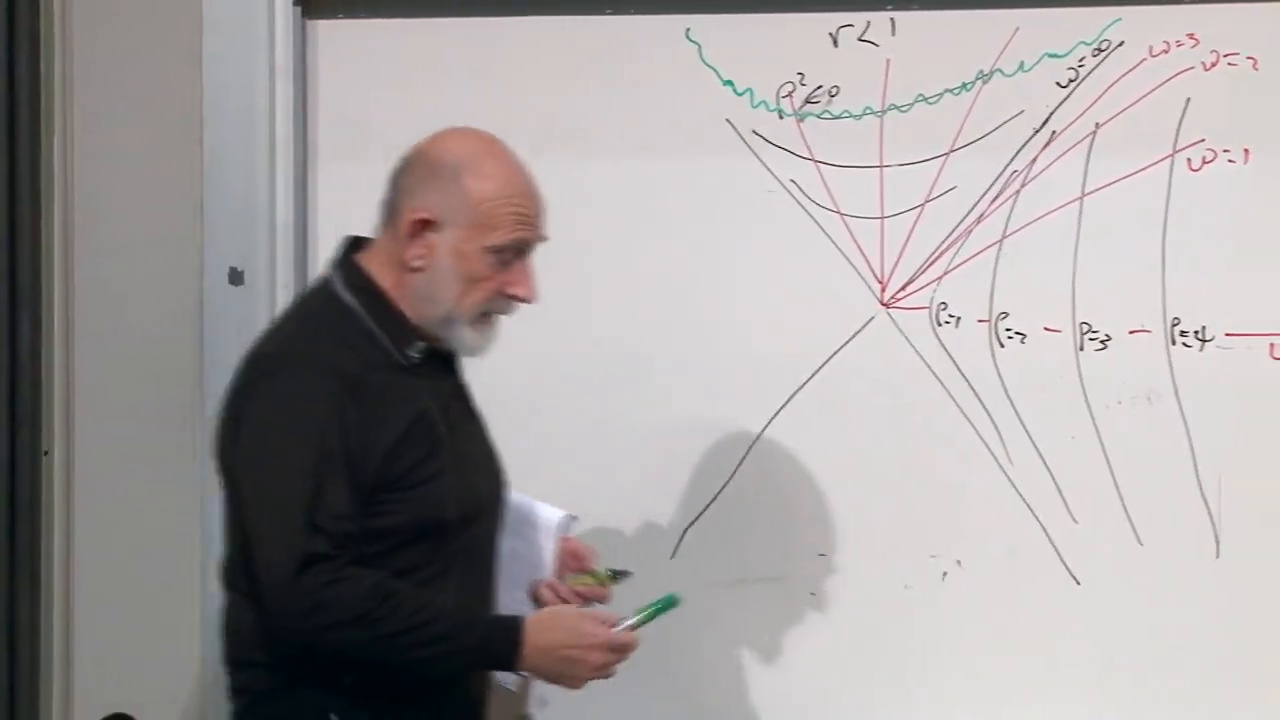
\includegraphics[width=0.88\textwidth]{lecture_07_figure_06.png}
\caption{完成したボード幾何：\(\rho\) 一定の双曲線、\(\omega\) 一定の光線、ヌル地平線、およびその上の \(r<1\) 領域。}
\lectureframe{00:38:30}
\end{figure}

\begin{figure}[htbp]
\centering
\resizebox{0.96\linewidth}{!}{%
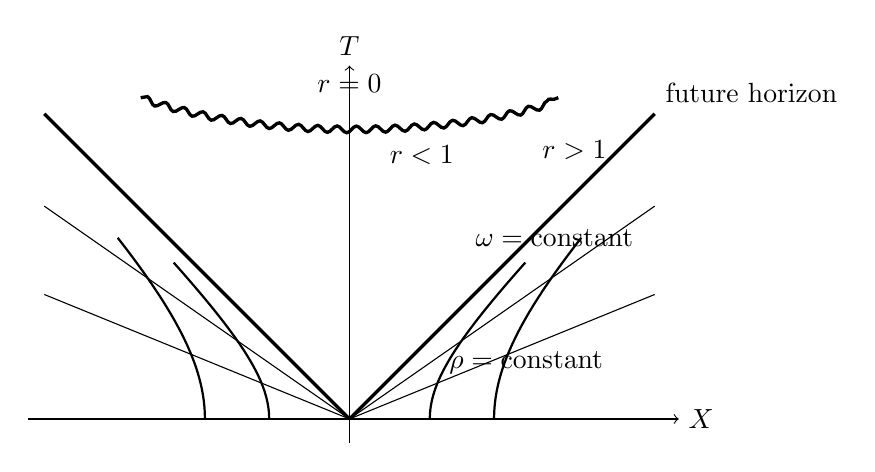
\begin{tikzpicture}[scale=1.02]
\draw[->] (-4.0,0) -- (4.1,0) node[right] {$X$};
\draw[->] (0,-0.3) -- (0,4.4) node[above] {$T$};
\draw[very thick] (0,0) -- (3.8,3.8)
  node[above right] {future horizon};
\draw[very thick] (0,0) -- (-3.8,3.8);
\draw[thick]
  plot[domain=0:1.42,samples=50]
  ({1.0*cosh(\x)},{1.0*sinh(\x)});
\draw[thick]
  plot[domain=0:1.05,samples=50]
  ({1.8*cosh(\x)},{1.8*sinh(\x)});
\draw[thick]
  plot[domain=0:1.42,samples=50]
  ({-1.0*cosh(\x)},{1.0*sinh(\x)});
\draw[thick]
  plot[domain=0:1.05,samples=50]
  ({-1.8*cosh(\x)},{1.8*sinh(\x)});
\draw[thin] (0,0) -- (3.8,1.55);
\draw[thin] (0,0) -- (3.8,2.65);
\draw[thin] (0,0) -- (-3.8,1.55);
\draw[thin] (0,0) -- (-3.8,2.65);
\draw[very thick,decorate,decoration={snake,amplitude=1.2pt,segment length=7pt}]
  (-2.6,4.0) .. controls (-1.2,3.5) and (1.2,3.5) .. (2.6,4.0);
\node at (0,4.18) {$r=0$};
\node at (2.2,0.7) {$\rho=\mathrm{constant}$};
\node at (2.55,2.25) {$\omega=\mathrm{constant}$};
\node at (0.9,3.28) {$r<1$};
\node at (2.8,3.35) {$r>1$};
\end{tikzpicture}
}
\caption{明快な因果的再構成。地平線はヌル線であり、一方、曲率特異点 \(r=0\) は穴の内部の未来境界である。}
\label{fig:l7-kruskal-clean}
\end{figure}

小さい \(\rho\) の極限は、ユークリッド極座標における小半径極限とは異なる。小さいユークリッド円は一点へ収縮する。\(\rho\) 一定の双曲線はヌル線全体に近づく。したがって \(\rho=0\) は、軸の交点だけでなく地平線全体を表す。

外部の公式は \(r<1\) へ解析接続できる。地平線の近くでは \(r-1\simeq\rho^2/4\) であるから、内部は形式的に \(\rho^2<0\) に対応する。\(\rho\) を虚数と呼んでもよいが、\(\rho^2\)、\(r\)、または正則座標 \(T,X\) を用いる方が明快である。内部ではシュヴァルツシルトの \(t\) と \(r\) の係数の符号が入れ替わる。それは物理的な腕時計が物差しになるという意味ではない。シュヴァルツシルト座標がその因果的性格を交換したという意味である。

\begin{classroomqa}
\audiencequestion{地平線の内部にある水平な双曲線とは何であり、直線的光線とは何か。}
\lecturerresponse{双曲線は \(r\) 一定、等価的には \(\rho^2\) 一定であり、\(r<1\) へ連続的に延びる。光線はシュヴァルツシルト時間一定である。外部ではそれらは有用な座標格子をなすが、内部では同じラベルを物理的な観測者軌道と誤認してはならない。
\lecturetimestamp{00:44:12--00:44:59}}
\end{classroomqa}

\begin{classroomqa}
\audiencequestion{垂直方向は時間座標か、そしてそれは誰の基準系を表すのか。}
\lecturerresponse{それは新しい時空図における正則な時間方向であるが、特異なシュヴァルツシルト時間 \(t\) ではない。この図は自由落下する因果構造に適合している。外部の固定半径に保持された観測者は双曲線に沿い、加速しなければならない。自由落下する観測者はヌル地平線を滑らかに横切る。
\lecturetimestamp{00:45:54--00:46:48}}
\end{classroomqa}

\begin{classroomqa}
\audiencequestion{内部で \(\rho^2<0\) なら、\(i\) の明示的な因子はどこにあるのか。}
\lecturerresponse{虚数の \(\rho\) を導入することもできるが、そうしても何も得られない。不変な内容は \(r\)、\(\rho^2\)、および実の正則座標 \(T,X\) によって担われる。関係 \(r-1\simeq\rho^2/4\) は地平線近傍展開にすぎない。
\lecturetimestamp{00:52:35--00:53:00}}
\end{classroomqa}

正則図は講義ではしばしばクルスカル図として説明される。厳密には、正確なクルスカル座標は完全なシュヴァルツシルト計量を正則に保つ動径因子を含むのに対し、式~\eqref{eq:l7-rindler-transform} はその地平線近傍形である。因果的メッセージは同じである。地平線は滑らかだが、内部の未来向き時間的またはヌル曲線はすべて \(r=0\) で終わる。超光速の向き転換によって地平線を通り抜けて戻ることはできない。

\subsection{座標特異点はいかに理解されたか}

地平線の滑らかさは、元のシュヴァルツシルト座標がその係数を特異に見せるため、歴史的に見るのが難しかった。エディントン、後にフィンケルシュタインが地平線を横切る座標を導入し、フィンケルシュタインは一方通行の因果的境界を認識した。座標変換に熟達していたクルスカルは、プラズマ物理学からその手腕を得て、永遠の解の大域的正則図を与えた。

講義は次にジョン・ホイーラーについてしばし止まる。彼は「ブラックホール」という言葉を避けがたいものにするのに貢献した。この停止は個人的なものでもあり歴史的なものでもある。ホイーラーは、核競争に関する判断を含む政治的判断が鋭く異なった場合でさえも、穏やかで思慮深い友人として記憶されている。ホイーラーが社会的に因習的であるという戯画に抗するために、ユーモラスな個人的逸話が語られる。技術的な論点は「ブラックホールには毛がない」という反論において戻ってくる。乱れた非回転の穴は急速に球対称へと落ち着く。回転する穴は、その保存されたパラメータによって固定された定常形状へと落ち着く。これは毛なしの考えの講義における定性的な版であり、完全な定理の証明ではない。

\section{アリスは横切る。ボブは外にとどまる}

最大拡張図には、通常の初期データから崩壊する星の単純な時空には現れない領域が含まれる。観測者実験では、外部、未来の地平線、そしてブラックホール内部のみを用いる。

\begin{figure}[htbp]
\centering
\includegraphics[width=0.84\textwidth]{lecture_07_figure_04.png}
\caption{アリスの落下する世界線と一定シュヴァルツシルト時間の光線。極限の光線は\(t=\infty\)とラベル付けされる。}
\lectureframe{00:54:54}
\end{figure}

アリスは自由落下する。彼女の世界線は地平線を横切り、有限の固有時間で特異点に到達する。ブラックホールが十分大きく、そこでの潮汐力が小さいならば、地平線において彼女の時計に特異なことは何も起こらない。

代わりにボブは固定された外部半径にとどまる。位置を保つには加速度が必要である。アリスの軌道の後の点からの光は、増大する遅延と増大する赤方偏移を伴って彼に届く。シュヴァルツシルト時間では、アリスは\(t=\infty\)に近づき、ボブは彼女の地平線横断後に放出された信号を決して受け取らない。これらは因果的信号と外部のスライスに関する記述であり、地平線における物質的表面の証拠ではない。

\begin{classroomqa}
\audiencequestion{もしボブがアリスが遅くなるのを見るなら、アリスはボブが速くなるのを見なければならないか？}
\lecturerresponse{いいえ。アリスは彼女の世界線が続く限り、ボブからの通常の光信号を受け取り続ける。ボブの世界線上で彼女に到達しうる最後の事象が存在するが、その事象が最後であるのは、アリスがその後特異点に衝突するからにすぎない。ボブに突然のことは何も起こらない。観測は常に過去の光円錐を覗き込み、二つの世界線は非対称な因果関係を持つ。
\lecturetimestamp{00:58:31--01:01:23}}
\end{classroomqa}

\begin{classroomqa}
\audiencequestion{もしボブが、アリスが彼の座標でまだ地平線の近くにいると知っているなら、彼は下に行き、彼女を回収して戻ることができるか？}
\lecturerresponse{救助の世界線は、アリスが事象の地平線を横切る前に彼女に会わなければならない。その事象の後、未来向きの経路は彼女に会って外部に戻ることはできない。シュヴァルツシルトのスライスが横断を\(t=\infty\)に置くという事実は、アリスが回収可能な物質的表面に座っているままであることを意味しない。それは、それらのスライスが地平線を越えた大域的な「今」の概念を与えないことを示している。
\lecturetimestamp{01:01:24--01:02:12}}
\end{classroomqa}

\section{チャーリーはアリスを追う}

チャーリーをアリスの少し後ろで落下させる。すると両者は地平線の近くで近似的に慣性系にある。彼らは信号を交換し、双方向に会話し、あるいは手をつなぐことさえできる。どちらも地平線を示す道標を見つけない。ボブとの対比は、三人の名を持つ人々の間の対比ではない。それは自由落下と、外部にとどまる加速された世界線との対比である。

\begin{classroomqa}
\audiencequestion{もしアリスが先に落ち、チャーリーがフープを追うバスケットボールのように続くなら、ボブは何を見るか？}
\lecturerresponse{ボブは両者が地平線に近づくのを見る。先にいるアリスは、まず次第に遅くなり半径方向に圧縮されて見える。チャーリーは彼女の後ろでますます近くに見えるが、ボブの極限的な外部の見方では決して彼女に追いつかない。この視覚的な積み重なりは、落下者のどちらが感じるかを記述していない。
\lecturetimestamp{01:04:12--01:06:05}}
\end{classroomqa}

\begin{classroomqa}
\audiencequestion{見かけの平坦化は、落下者を半径方向に伸ばすはずの潮汐力と矛盾しないか？}
\lecturerresponse{それらは異なる効果である。平坦化はボブのシュヴァルツシルト座標による記述に属する。潮汐的伸長は、アリスとチャーリーが感じることのできる局所的な曲率効果である。観測者の議論は、地平線での潮汐効果が無視できるほど十分に大きなブラックホール、または十分に小さな観測者を仮定している。およそ太陽質量の穴は代わりに激しい地平線潮汐を持つが、超大質量のものは弱い地平線潮汐を持ちうる。
\lecturetimestamp{01:06:07--01:08:18}}
\end{classroomqa}

\begin{classroomqa}
\audiencequestion{チャーリーは、自分がまだ外にいる間に、アリスが横切るのを見るか。}
\lecturerresponse{ヌル光線を描け。アリスの横断時に放出された光は地平線に沿って進み、チャーリーが横断するときにチャーリーに到達する。その事象において、彼は自分が彼女の横断を見たと計算できる。ただし、どちらの観測者も局所的な目印に出会うわけではない。その後、彼は彼女が内側にいるのを見ることができる。もし彼が横断する前に加速して離れ、外にとどまることに成功すれば、彼はその横断を決して見ない。
\lecturetimestamp{01:08:19--01:11:11}}
\end{classroomqa}

\begin{classroomqa}
\audiencequestion{アリスがすでに内側にいて、チャーリーが外側にいる場合、彼らの後の半径と横断時刻をどのように比較できるのか。}
\lecturerresponse{「同じ時刻に」といった表現から読み取れるような、観測者に依存しない同時性の関係は存在しない。アリスは自分の過去光円錐上にチャーリーを見ており、彼の後の横断を見ることができるのは、彼女がさらに内側にいるときだけである。具体的な世界線とヌル光線がこの問いに答える。多数の大きく離れた落下者への広範な外挿は、一つの普遍的な横断時刻を仮定するのではなく、彼らの実際の因果図を描くことによって確認しなければならない。
\lecturetimestamp{01:11:14--01:12:31}}
\end{classroomqa}

正則な地平線近傍座標では、自由落下軌道はほぼ直線である。完全なシュヴァルツシルト幾何学では厳密に直線ではないが、大きく弱く曲がった地平線の近くでは近似が良くなる。

\begin{classroomqa}
\audiencequestion{弦理論は、ブラックホール内部の量子重力領域で何が起こるかを決着させられるのか。}
\lecturerresponse{まさにそこが、この主題が微妙になる場所である。特異点の近くでは重力の量子論が必要であり、弦理論は候補となる枠組みであるが、関連する問いは古典的な図の単純な適用によって解決されたのではなく、活発で困難なものであった。
\lecturetimestamp{01:13:04--01:13:38}}
\end{classroomqa}

\begin{classroomqa}
\audiencequestion{アリス自身の時計と速度は、彼女が横切るときにどうなるのか。}
\lecturerresponse{彼女の時計は通常の局所的速さで刻み続け、有限の固有時を記録する。彼女の瞬間静止系では彼女は静止しており、局所的な自由落下系に対しては通常の有限の速度をもつ。大きな地平線の近くでは幾何学はほとんど平坦であるため、彼女の世界線に沿った等固有時目盛りは、特異点の近くで曲率が強くなるまで正則なままである。
\lecturetimestamp{01:13:39--01:14:44}}
\end{classroomqa}

\begin{classroomqa}
\audiencequestion{ボブが外向きに加速するが、落下して通り抜けるのを避けるほど十分強くは加速しない場合はどうなるか。}
\lecturerresponse{その場合、彼の世界線は外向きに曲がるが、それでも地平線を横切る。もし彼が非常に遅く横切るなら、彼はアリスの横断直後に彼女を見ることができるが、特異点までの残りの固有時は短い。スケッチ上の世界線の傾きは較正された物差しや時計ではない。生き残るのは因果的順序であり、描かれたユークリッド的長さではない。
\lecturetimestamp{01:14:47--01:16:31}}
\end{classroomqa}

これらの結論はすべて、光を追い越す信号はないと仮定している。講義では、当時イタリアで報道された一見超光速の中性子に関する最近の報道について短く冗談を言う。これは相対性理論の例外ではなく、実験的なタイミング誤差への言及である。因果的構成自体はヌル線によって境界づけられたままである。

\begin{classroomqa}
\audiencequestion{アリスとボブが運ぶ同期した時計は、アリスが地平線に向かって飛び込み、戻ってくる場合にこの問題を決着させられるか。}
\lecturerresponse{彼らは一致したときに時計を比較できるが、彼らの世界線が分かれた後には、特に一方が運動を変えるときには、一意な遠方同期は存在しない。両方の世界線と交換されるヌル光線を描け。その図が、指定された任意の実験に対する操作的答えを与える。
\lecturetimestamp{01:17:34--01:18:25}}
\end{classroomqa}

\begin{figure}[htbp]
\centering
\includegraphics[width=0.86\textwidth]{lecture_07_figure_05.png}
\caption{アリス、ボブ、チャーリーの問いに答えるために用いられた累積的因果図。各観測は、観測された事象から観測者の世界線へヌル光線をたどることによって位置づけられる。}
\lectureframe{01:18:12}
\end{figure}

\begin{figure}[htbp]
\centering
\resizebox{0.96\linewidth}{!}{%
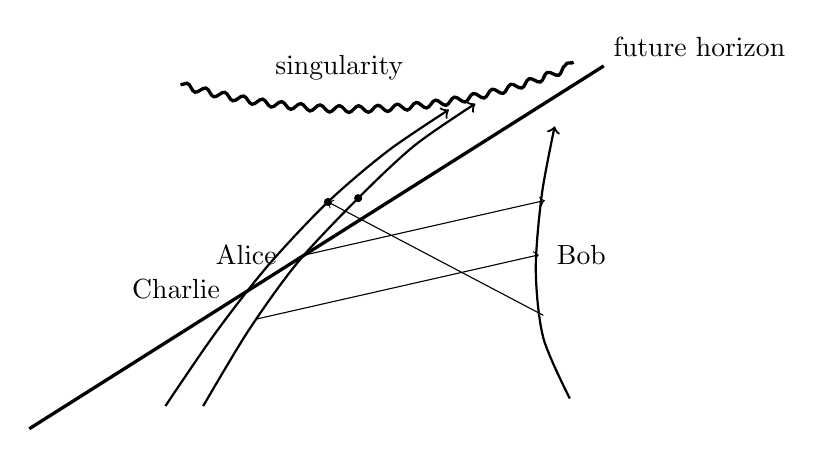
\begin{tikzpicture}[scale=0.96]
\draw[very thick] (-3.8,-0.3) -- (3.8,4.5);
\node[above right] at (3.8,4.5) {future horizon};
\draw[very thick,decorate,decoration={snake,amplitude=1.2pt,segment length=7pt}]
  (-1.8,4.25) .. controls (0.1,3.72) and (2.0,3.92) .. (3.4,4.55);
\node at (0.3,4.48) {singularity};
\draw[thick,->]
  plot[smooth] coordinates {(-1.5,0.0) (-0.9,1.0) (-0.25,1.9)
  (0.55,2.75) (1.3,3.45) (2.1,4.0)};
\node[left] at (-0.4,2.0) {Alice};
\draw[thick,->]
  plot[smooth] coordinates {(-2.0,0.0) (-1.35,0.95) (-0.65,1.85)
  (0.15,2.7) (0.95,3.38) (1.75,3.92)};
\node[left] at (-1.15,1.55) {Charlie};
\draw[thick,->]
  plot[smooth] coordinates {(3.35,0.1) (3.0,0.9) (2.9,1.8)
  (2.98,2.8) (3.15,3.7)};
\node[right] at (3.05,2.0) {Bob};
\draw[thin,->] (-0.8,1.15) -- (2.94,2.0);
\draw[thin,->] (-0.15,2.0) -- (3.02,2.72);
\draw[thin,->] (3.0,1.2) -- (0.15,2.7);
\draw[fill] (0.55,2.75) circle (1.3pt);
\draw[fill] (0.15,2.7) circle (1.3pt);
\end{tikzpicture}
}
\caption{概略的な観測者図。ボブの外部観測と、アリスとチャーリーの相互観測は、相互的な時計のスローガンではなく、異なるヌル光線構成である。}
\label{fig:l7-observers-clean}
\end{figure}

\begin{classroomqa}
\audiencequestion{ボブはアリスを無限の時間にわたって見るのか、そしてそれは彼の実在において彼女が決して死なないことを意味するのか。}
\lecturerresponse{ボブは彼の時間の非有界な区間にわたって彼女の信号を受け取るが、彼女の時計がゼロの速さに向かって遅くなるのを見、彼女の横断前に放出された有限個の心拍の系列だけを受け取る。「実在」という語は、局所的な事象と観測者の漸近的記録との区別を隠している。アリスは地平線で止まった時計を経験しない。ボブの記録はますます遅延し赤方偏移する。
\lecturetimestamp{01:18:32--01:20:59}}
\end{classroomqa}

\begin{classroomqa}
\audiencequestion{アリスは地平線を越えたとたん、地平線上に凍りついて見えていた古い物質のすべてを突然見るのだろうか。}
\lecturerresponse{突然視界が晴れるということは起こらない。落下するにつれて、それ以前の物質を見るための過去光円錐は連続的に変化する。今自分に届いている光は以前に放出されたものであり、その物質は自分の前を横切ったのだと彼女は推論できる。アリスに対するチャーリーの見方も同じ教訓を与える。どちらの横断も局所的な不連続を生じさせたり、隠された椅子や恐竜の山を明らかにしたりはしない。
\lecturetimestamp{01:21:02--01:23:48}}
\end{classroomqa}

\begin{classroomqa}
\audiencequestion{落下する者に何が見えるかについて、現実的なシミュレーションはあるのだろうか。}
\lecturerresponse{講義はアンドリュー・ハミルトンのブラックホール可視化を指し示している。それらは入射光の激しい光行差と周波数偏移を伝えることができるが、表示は啓発というより当惑させるものかもしれない。「地平線では何も特別なことはない」とは局所的な幾何学についてのことであり、見た目が普通の空についてのことではない。
\lecturetimestamp{01:24:11--01:25:29}}
\end{classroomqa}

\section{永遠の穴から成長する穴へ}

最大に拡張された永遠の図の下側の頂点は、恒星の崩壊によって形成されたブラックホールにとって直接的な意味をほとんど持たない。外部、未来の地平線、未来の内部を含む部分だけが、単純な崩壊の幾何学に現れる。この区別は、物質が穴の質量を変えることが許されるときに本質的になる。

\begin{classroomqa}
\audiencequestion{理想化された図の下側の頂点は、どのような物理的出来事を表しているのか。}
\lecturerresponse{永遠の数学的解にとって、それは最大拡張の一部である。崩壊する物質から形成されたブラックホールは、その下側の領域全体を含まない。その地平線には形成の歴史があり、それには異なる大域的図が必要であり、次の講義で展開される。
\lecturetimestamp{01:25:59--01:26:52}}
\end{classroomqa}

小さな試験物体が落下するとき、その反作用は無視でき、固定されたシュヴァルツシルト図で十分である。実質的な質量が落下すると、ブラックホールの質量とシュヴァルツシルト半径が増大する。
\begin{equation}
r_{\mathrm S}=2GM,
\qquad
\Delta r_{\mathrm S}=2G\,\Delta M.
\label{eq:l7-growing-radius}
\end{equation}
地平線は入射する物体に向かって変形し、地平線は結合し、歪んだ共通の地平線は急速に落ち着く。講義の非回転の理想化では、終点はわずかに大きな球である。実際の合体も重力波としてエネルギーを放射し、一般には回転する穴を残す。

\begin{classroomqa}
\audiencequestion{質量が落下すると地平線が成長するなら、古い地平線の近くで凍りついて見えた物質に会うために外側へ動くのだろうか。}
\lecturerresponse{十分に大きな質量の落下物体に対しては、試験粒子の描像はもはや有効でない。地平線は変形し、入射する物体のトラップされた領域と結合し、より大きな定常な地平線へと緩和する。事象の地平線の正確な位置は大域的であり、落下する物質が到着する前の領域にまで及ぶことがある。講義は完全な構成を意図的に次の会合へ延期している。
\lecturetimestamp{01:26:55--01:29:05}}
\end{classroomqa}

\begin{classroomqa}
\audiencequestion{物質が地平線に到達するのに無限のシュヴァルツシルト時間がかかると言われるのに、なぜ天文学者は閃光を見ることができるのか。}
\lecturerresponse{明るい放射は地平線そのものから来るのではない。降着流や円盤の中のガスは地平線の外側で衝突し加熱される。強い光子軌道の近くも含めてである。その外部のプラズマは我々に届く光を放出しうる。空のシュヴァルツシルト幾何学は因果の問題を切り離すが、天体物理的環境の完全なモデルではない。
\lecturetimestamp{01:29:07--01:30:22}}
\end{classroomqa}

特徴的な緩和時間は光の横断時間によって決まる。
\begin{equation}
t_{\mathrm{cross}}\sim\frac{r_{\mathrm S}}{c},
\qquad
t_{\mathrm{relax}}\sim
\text{a few to a few tens of }t_{\mathrm{cross}}.
\label{eq:l7-relaxation-scale}
\end{equation}
講義は\(10^{-5}\,\mathrm{s}\)をキロメートル規模の穴の横断時間と見積もり、小さな合体がほぼ定常になるまでおよそ\(10^{-3}\,\mathrm{s}\)と見積もっている。十億太陽質量の穴では、対応する時間は分から時間の単位で測られる。これらはスケーリングの見積もりであり、精密な合体計算ではない。幾何学的な系列が要点である。ダンベル、ピーナッツ、ほぼ球形、定常。

\begin{classroomqa}
\audiencequestion{歪んだ、あるいは新たに合体した地平線はどれくらい速く落ち着くのか。}
\lecturerresponse{光が穴を横切るのに要する時間よりそれほど長くない時間スケールで。すべての長さと時間は\(r_{\mathrm S}\)とともにスケールするので、小さな穴は一秒の何分の一かで落ち着き、超大質量の穴ははるかに長い時計時間で落ち着く。ノーヘアの言明は定常な終点を記述する。過渡的な変形は重力放射を通じてエネルギーを運び去る。
\lecturetimestamp{01:30:26--01:33:18}}
\end{classroomqa}

\begin{classroomqa}
\audiencequestion{古い地平線と新しい地平線の間に以前の物質が存在し、その間に別の重い天体が落下する場合、ボブには何が見えるか。}
\lecturerresponse{その問いは、二つの静的シュヴァルツシルト図を継ぎ合わせることで首尾一貫して答えることはできない。時間依存の崩壊幾何を解くか構成し、その大域的地平線を特定しなければならない。講義はこの問いを保持し、その答えを地平線形成が主題となる次週に明示的に先送りする。
\lecturetimestamp{01:33:20--01:35:41}}
\end{classroomqa}

\section{スケールが変わると何が変わるか}

\(r_{\mathrm S}\)が変化しても無次元図は変化しない。しかし、描かれた間隔の物理的意味は変化する：
\begin{equation}
d\tau_{\mathrm{physical}}^2
=
r_{\mathrm S}^2\,d\hat{\tau}^2,
\qquad
\ell_{\mathrm{physical}}
=
r_{\mathrm S}\,\hat{\ell}.
\label{eq:l7-scale-restoration}
\end{equation}
キロメートル規模の穴に対して半キロメートルを表す無次元の間隔は、十億倍大きな穴に対してはおよそ五億キロメートルを表す。等しく描かれた球との類推が再び戻ってくる：形状は変わらないが、一本の線が表すメートル尺の数は半径に比例してスケールする。

\begin{classroomqa}
\audiencequestion{シュヴァルツシルト半径が変化すると、因果図はどのように変化するか。}
\lecturerresponse{半径をスケールアウトした後は変化しない。図に割り当てられたすべての物理的長さと時間は\(r_{\mathrm S}\)倍され、対応する無次元点における曲率は\(r_{\mathrm S}^{-2}\)倍される。
\lecturetimestamp{01:35:41--01:38:10}}
\end{classroomqa}

\begin{classroomqa}
\audiencequestion{ボブが一つの角度位置でホバリングする代わりに周回する場合、因果的結論は変化するか。}
\lecturerresponse{詳細な赤方偏移と到来方向はより複雑になるが、地平線の因果的分離は変化しない。地平線の内部から放出された信号を受け取る外部の時間的軌道は存在しない。
\lecturetimestamp{01:38:12--01:38:26}}
\end{classroomqa}

\begin{classroomqa}
\audiencequestion{球対称殻の内部では重力が消えるのだから、ブラックホールの質量がその表面に広がっているために地平線の内部でも重力は消えるのか。}
\lecturerresponse{いいえ。事象の地平線は質量を担う物質的な殻ではない。したがって、ニュートンの殻定理はそれには適用されない。講義は静的 exterior 解を曲率特異点にある点源と比較するが、形成中に現在落下している物質は次回の講義に先送りされた時間依存幾何を必要とする。
\lecturetimestamp{01:38:28--01:40:41}}
\end{classroomqa}

\section{回転と動径幾何}

角運動量は崩壊を生き延びる。回転するブラックホールはシュヴァルツシルトとは異なる外部幾何を持ち、その定常解はカー解であり、回転は地平線の幾何を歪め、慣性系の引きずりは慣性方向を穴の周りに運ぶ。原理的には、角運動量はそれらの外部重力効果から測定される。角運動量を持つ物質は、地平線を横切るだけでそれを失うことはない。

\begin{classroomqa}
\audiencequestion{ブラックホールは測定可能な角運動量を持ち得るか、また回転はその外部の重力を変えるか。}
\lecturerresponse{はい。角運動量は保存されたパラメータとして残り、定常幾何を変形させ、慣性系の引きずりを生じさせる。地平線はもはや単純な球対称シュヴァルツシルト地平線ではない。講義はその歪みを地球の扁平な形状と定性的に比較しつつ、完全な回転解はかなり複雑であると注記する。
\lecturetimestamp{01:40:45--01:42:36}}
\end{classroomqa}

\begin{classroomqa}
\audiencequestion{\(r\)と固有距離\(\rho\)の関係は、重力が空間を収縮させることを意味するのか。}
\lecturerresponse{固有動径距離\(\rho\)は単位地平線の外側で
\begin{equation*}
\frac{d\rho}{dr}=\sqrt{\frac{r}{r-1}}>1
\end{equation*}
を満たす。したがって、与えられた座標増分\(dr\)は地平線近くでより大きな固有動径間隔に対応する。空間が収縮しているか引き伸ばされていると言うことは、どの座標間隔を比較しているかに依存する。不変な言明は固有距離の関係そのものである。
\lecturetimestamp{01:42:36--01:43:20}}
\end{classroomqa}

\section{最終的な質問}

\begin{classroomqa}
\audiencequestion{ボブの視点ではアリスの時計は停止に近づく。アリスの視点では、ボブの空間または時間は終わりを迎えるのか。}
\lecturerresponse{いいえ。アリスは自身の世界線が終わるまで、ボブの世界線上にある successive な事象からの通常の信号を見る。彼女がそれ以降のボブの事象を見ないのは、彼女の世界線上にそれ以降の点が存在しないためであり、ボブや彼の空間が消えるためではない。これらの正則な因果座標では動径ヌル光線は直線的に描かれる。別の座標系で曲がった経路として現れることは、それらが結ぶ事象を変えない。
\lecturetimestamp{01:43:21--01:45:20}}
\end{classroomqa}

一般相対性理論は二つの相補的な課題を提示する。計量が与えられれば、測地線とヌル光線をたどって観測者が何を測定するかを決定できる。物質の分布が与えられれば、アインシュタイン方程式を解いて計量を見出さなければならない。第一の課題はこの講義で扱われた。第二の課題は通常より難しく、対称的な崩壊が扱いやすい例を提供するとはいえ、そうである。

\begin{classroomqa}
\audiencequestion{蒸発するブラックホールの事象の地平面と特異点はどうなるのか。}
\lecturerresponse{講義では、地平面が収縮して特異領域の端点と出会うという模式的な描像が示される。蒸発は半古典的な量子過程であり、最終的なプランクスケールの端点は古典的なシュヴァルツシルト図では決着しない。したがって、収縮するスケッチは定性的な予告編として読むべきであり、完全な量子幾何学ではない。
\lecturetimestamp{01:46:04--01:46:32}}
\end{classroomqa}

ほとんどすべての天体物理的ブラックホールは回転しているはずである。恒星はすでに角運動量を持っており、重力崩壊は、スケート選手が腕を引き寄せるおなじみの仕方でその角速度を増幅する。カー・ブラックホールの特異構造は、ここに描かれたシュヴァルツシルトの\(r=0\)面ではなく、物質が文字通り無限の線速度で回転していると記述すべきものではない。

\begin{classroomqa}
\audiencequestion{回転しない巨視的ブラックホールは一般的なのか、またブラックホールはどれくらい存在するのか。}
\lecturerresponse{角運動量が厳密にゼロであることは例外的な理想化であろう。講義は宇宙全体の個数について、銀河の数と恒星の数の間のどこか、おそらく\(10^{15}\)程度という、桁程度の教室での推測しか与えていない。それは講義当時の推定であり、測定された統計ではない。確かな点は、重力崩壊が一般に何らかの角運動量を保存し増幅するということである。
\lecturetimestamp{01:46:32--01:48:42}}
\end{classroomqa}

\begin{classroomqa}
\audiencequestion{ブラックホールは既存の物質から形成されるのか、それとも量子過程を通じて現れるのか。}
\lecturerresponse{通常の天体物理的ブラックホールは、既存の恒星物質が重力崩壊するときに形成される。核燃焼とエネルギーの外向きの流れが恒星を支えるのに寄与する。燃料が尽きると、残骸は収縮する。その質量と利用可能な圧力の支え方に応じて、白色矮星になるか、中性子星になるか、あるいは崩壊を止める支えがなければ、自身のシュヴァルツシルト半径の内側に入り、ブラックホールを形成する。
\lecturetimestamp{01:48:43--01:50:23}}
\end{classroomqa}

\begin{classroomqa}
\audiencequestion{微視的ブラックホールは形成されうるのか、またその寿命と最小サイズを決めるものは何か。}
\lecturerresponse{この部分は推測的である。ホーキング蒸発は質量が小さいほど速く、寿命はおよそ\(M^3\)に比例してスケールする。講義では、寿命が宇宙論的でありうるブラックホールについて山ほどの質量との比較を用いているが、その数値的な類推は粗いものでしかない。初期宇宙における激しい密度揺らぎや、十分に高エネルギーの衝突が、考えうる形成機構である。およそ\(10^{-5}\,\mathrm{g}\)のプランク質量に近いブラックホールは、古典的な幾何学的記述が信頼できなくなるスケールを示す。通常の加速器でそのエネルギーに到達するには、素直な外挿のもとでは信じがたいほど大きな機械が必要であろうが、形成の主張自体は原理的には可能である。
\lecturetimestamp{01:50:23--01:53:31}}
\end{classroomqa}

\begin{classroomqa}
\audiencequestion{この講義は宇宙論、暗黒物質、暗黒エネルギー、エントロピー、重力波まで到達するのか。}
\lecturerresponse{宇宙論的応用、そしておそらく重力波は、後の話題として残りうる。ブラックホールのエントロピーは四半期を超えて先送りされる。講義は、その晩に計画された内容のおよそ四分の一しか扱えなかったことを認めて終わる。すなわち、質問を注意深く解決することのほうが、概要を駆け足で進むことよりも重要なのである。
\lecturetimestamp{01:53:33--01:54:38}}
\end{classroomqa}

操作上の規則は、その場のあらゆる質問を生き延びる。世界線を指定し、ヌル光線を描き、それらが結ぶ事象を特定する。地平面は局所的な物理が破れる場所ではなく、すべての未来向きの信号がその内側にとどまる境界である。次の講義では、永遠の背景を崩壊する源に置き換え、その境界がどのように形成されるかを示す。
